\documentclass[10pt,a4paper,titlepage]{jreport} % ドキュメントクラスを1つに統一


\usepackage[top=25truemm,bottom=25truemm,left=20truemm,right=20truemm]{geometry} % 余白設定
\usepackage[dvipdfmx]{graphicx} % 画像の挿入
\usepackage{graphicx}
\usepackage{listings} % コードリスト用
\usepackage{jlisting} % 日本語対応のリスト用
\usepackage{jverb} % 日本語のベタ打ち
\usepackage{booktabs}
\usepackage{pgfplots} % グラフ描画用パッケージ
\pgfplotsset{compat=1.18} % バージョン指定

\parindent = 0pt % 段落の字下げを無効化

\usepackage{titlesec}
\usepackage{etoolbox}
\makeatletter
\patchcmd{\chapter}{\if@openleft\cleardoublepage\else\if@openright\cleardoublepage\else\clearpage\fi\fi}{}{}{}
\makeatother
\lstset{breaklines=true, postbreak=\mbox{$\hookrightarrow$}\space, keepspaces=true, escapeinside={\%*}{*)}}

\titleformat{\chapter}[hang] % 章のフォーマットを変更
  {\normalfont\huge\bfseries} % フォント設定
  {\thechapter} % 番号部分の表示形式
  {1em} % 番号とタイトルの間のスペース
  {} % タイトルの前に入れる内容（ここでは空）
\usepackage{xcolor}
\usepackage{amsmath}
\usepackage{amssymb} % ←これで \mathbb{R} が使える

\lstset{
  language=Matlab,              % 言語はMATLAB
  basicstyle=\ttfamily\small,   % フォントは等幅、サイズ小さめ
  keywordstyle=\color{blue},    % キーワード（function, endとか）を青
  commentstyle=\color{green!50!black}, % コメントを深緑
  stringstyle=\color{red!70!black},    % 文字列（'...'）を赤系
  numbers=left,                 % 行番号を左に表示
  numberstyle=\tiny\color{gray},% 行番号をグレーで小さく
  stepnumber=1,                 % 毎行行番号つける
  numbersep=10pt,               % コードとの間隔
  backgroundcolor=\color{gray!10}, % 背景うっすらグレー
  frame=single,                 % 枠をつける
  rulecolor=\color{black},      % 枠線は黒
  breaklines=true,              % 長い行を折り返す
  breakatwhitespace=false,      % スペースでだけ折り返すか（falseにして自然な折り返し）
  showspaces=false,             % スペースは特別に表示しない
  showstringspaces=false,       % 文字列中のスペースも普通に表示
  tabsize=2                     % タブ幅2
}


\title{C102「AI・機械学習：ニューラルネットワークによる教師あり学習」} % タイトル
\author{
  学生番号：242C2016  氏名：奥村直 \\
  \\
  知的システム工学科システム制御コース
  } % 著者
\date{\today} % 日付

\begin{document}

\maketitle

\chapter{目的}

　本演習の目的は、実際にMatlabのプログラミングを行うことにより、AI・機械学習の基
礎の一つである「ニューラルネットワークによる教師あり学習」を理解することである。

\chapter{第１週：最急降下法}

　この演習では、Matlabで最急降下法のプログラミングを行うことにより、最急降下法を理解する。
また、Matlabのプログラミングに慣れることもここでの演習の目的とする。

\section{理論}

\subsection{学習}

　「学習」とは、学習の目的に合わせた損失関数を設定し、その損失関数を最小化するような
（学習）パラメータの値を求めることである。別の言い方をすると、設定した損失関数を最小化
するために行う（繰り返し）計算の過程を「学習」と呼ぶ。また、学習には大別して「教師あり学習」
と「教師なし学習」がある。

\subsection{最適化}

　最適化とは、最小化あるいは最大化したい目的関数と呼ばれる関数の値を最小あるいは最大にする変数（決定変数と呼ぶ）
の値を求めることである。

\subsection{勾配法}

　勾配法とは、目的関数の勾配情報を用いた最適化手法である。

\subsection{最急降下法}

　特に、最急降下法は勾配法の中でも代表的な手法である。

\section{変数が一つの関数に対する最急降下法}

上記の概説に従って演習課題を完成させる。

決定変数 $w \in \mathbb{R}$ に対する目的関数を考える。

\begin{equation}
L(w) = \frac{w^4}{20} - w^2 + w + 10
\end{equation}

この目的関数の勾配は次のようになる。

\begin{equation}
\frac{\partial L(w)}{\partial w} = \frac{w^3}{5} - 2w + 1
\end{equation}

この目的関数に対して最急降下法を適用するプログラムを作成する。
以下の手順1～4に従い、プログラミングを進める。

\subsection{関数のグラフを描く}

\begin{lstlisting}[caption=saikyu11]
%%%%% 以下を入力 %%%%%
% プログラム1.1: saikyou11.m
%
% 1変数の目的関数に対する最急降下法
%
% すべての変数の値を初期化する。グラフをすべて閉じる。
clearvars, close all
% (A)
% 
%% 目的関数のグラフを描く。
% w： 変数、範囲：-5.2から0.1刻みで5.2までの範囲
% Lw: 目的関数の値
w = -5.2:0.1:5.2;
Lw = obj_func(w);
plot(w, Lw, 'b-', 'LineWidth', 1.5), grid on, hold on
xlabel('w'), ylabel('L(w)')
set(gca, 'FontSize', 16) % フォントサイズを16ポイントにする
% (B)
%
%% 目的関数（objective function）の計算
function y = obj_func(w)
y = w.^4/20 - w.^2 + w + 10;
end
% (C)
%%%%% 以上を入力 %%%%%
\end{lstlisting}

\subsection{プログラムの説明}

\subsubsection{目的関数の計算}

同じファイル内で、functionを定義すると、そのファイル内で使える
関数定義となる。function y = obj＿func(w) は目的関数を計算する
関数、引数wはスカラーでも配列でもよい。yはwに対する関数の値であり、
wがスカラーの場合はスカラーを返し、wが配列の場合は配列を返す。

\subsection{完成後のプログラム}

\begin{lstlisting}[caption=saikyu11]
%%%%% 以下を入力 %%%%%
% プログラム1.1: saikyu11.m
%
% 1変数の目的関数対する最急降下法
%
% すべての変数の値を初期化する．グラフをすべて閉じる．
clearvars, close all
% ← (A)
w = 4;
ep = 0.1;
iters = 20;
ws = w;
for k = 1:iters
    g = grad(w);
    w = w - ep*g;
    ws = [ws; w];
end
%
%% 目的関数のグラフを描く
% w: 変数．範囲：-5.2から0.1刻みで5.2までの範囲
% Lw: 目的関数の値
w = -5.2:0.1:5.2;
Lw = obj_func(w);
plot(w, Lw, 'b-', 'LineWidth', 1.5), grid on, hold on
xlabel('w'), ylabel('L(w)')
set(gca, 'FontSize', 16) % フォントサイズを16ポイントにする．
% ← (B)
for k = 1:iters
    yk = obj_func(ws(k));
    plot([ws(k), ws(k)], [0, yk], 'rx--', 'LineWidth', 1.5);
end
%
%% 目的関数（objective function）の計算
function y = obj_func(w)
y = w.^4/20 - w.^2 + w + 10;
end
% ← (C)
function g = grad(w)
g = w.^3/5 - 2*w + 1;
end
%%%%% 以上を入力 %%%%%
\end{lstlisting}

\subsection{実行結果（グラフ）}

実行して得られたグラフを図2.1:saikyu11に示す。

\begin{figure}[htbp]
  \centering
  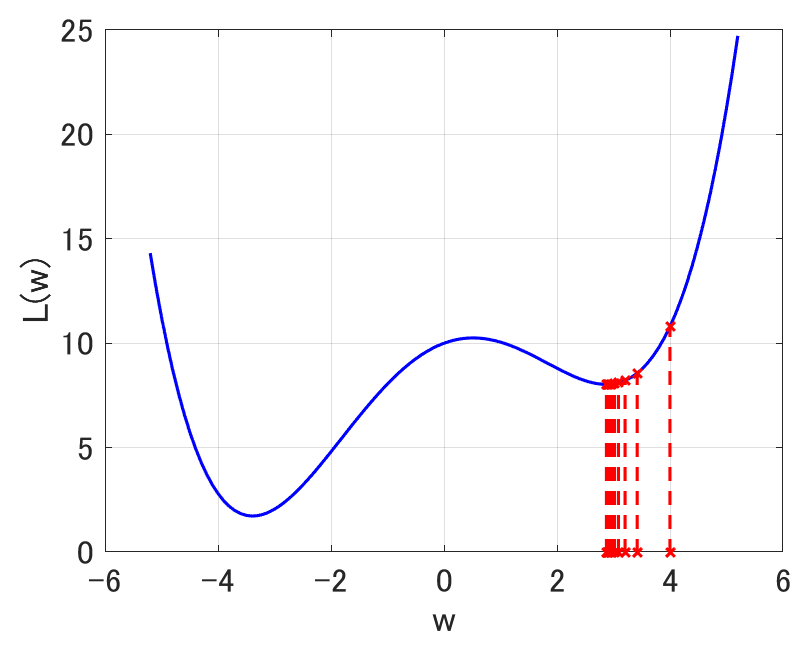
\includegraphics[width=0.8\linewidth]{saikyu11.eps}
  \caption{saikyu11}
  \label{fig:sample}
\end{figure}



\section{演習課題1.1}

\subsection{演習課題（a）}

（a）初期値wやステップ幅epを様々な値に変更し、最急降下法での収束
がどのように変わるか確かめよ。初期値は描画範囲（-5～5の範囲）で2
刻みくらいで変更する。ステップ幅epは0.8, 0.5, 0.2, 0.1, 0.05, 
0.01 などに変更する。必要に応じて、反復回数itersも変更する。\\

\subsection{演習課題1.1（b）}

（b）目的関数が

\begin{equation}
L(w) = \sin (2w) + \frac{w^2}{8} + 2
\end{equation}

の場合について、プログラムを変更して「saikyu12.m」とし、(a)と同じように
様々な初期値とステップ幅に対してどのような振る舞いになるかを確かめよ。
この場合の勾配 $\frac{ \partial }{ \partial w} L(w)$ は自分で計算すること。

目的関数 $L(w)$ の勾配を求めると、

\begin{equation}
\frac{ \partial }{ \partial w} L(w) = 2\cos{2w} + \frac{w}{4}
\end{equation}

であることが分かるから、saikyu11.mの

\begin{verbatim}
function g = grad(w)
g = w.^3/5 - 2*w + 1;
end
\end{verbatim}

の関数を以下のように変更し、

\begin{verbatim}
function g = grad(w)
g = 2 * cos(2 * w) + w/4;
end
\end{verbatim}

saikyu12.mの全体のソースコードを次に示す。

\begin{lstlisting}[caption=saikyu12]
  %%%%% 以下を入力 %%%%%
% プログラム1.1: saikyu11.m
%
% 1変数の目的関数対する最急降下法
%
% すべての変数の値を初期化する．グラフをすべて閉じる．
clearvars, close all
% ← (A)
w = 4;
ep = 0.1;
iters = 20;
ws = w;
for k = 1:iters
    g = grad(w);
    w = w - ep*g;
    ws = [ws; w];
end
%
%% 目的関数のグラフを描く
% w: 変数．範囲：-5.2から0.1刻みで5.2までの範囲
% Lw: 目的関数の値
w = -5.2:0.1:5.2;
Lw = obj_func(w);
plot(w, Lw, 'b-', 'LineWidth', 1.5), grid on, hold on
xlabel('w'), ylabel('L(w)')
set(gca, 'FontSize', 16) % フォントサイズを16ポイントにする．
% ← (B)
for k = 1:iters
    yk = obj_func(ws(k));
    plot([ws(k), ws(k)], [0, yk], 'rx--', 'LineWidth', 1.5);
end
%
%% 目的関数（objective function）の計算
function y = obj_func(w)
y = sin(2 * w) + w.^2/8 + 2;
end
% ← (C)
function g = grad(w)
g = 2 * cos(2 * w) + w/4;
end
%%%%% 以上を入力 %%%%%
\end{lstlisting}

\section{変数が二つの関数に対する最急降下法}

決定定数 $W = (w_1, w_2) \in \mathbb{R}^{1 \times 2} $ に対する次の目的関数を考える。

\begin{equation}
L(W) = \frac{w_1^4}{24} + \frac{w_2^4}{32} - w_1^2 - w_2^2 + w_1 + w_2 + 25
\end{equation}

この目的関数の勾配は次のようになる。

\begin{equation}
\frac{ \partial }{ \partial W} \partial L(W) = ( \frac{ \partial }{ \partial w_1 } L(W), \frac{ \partial }{ \partial w_2 } L(W))
\end{equation}

勾配 $ \frac{ \partial }{ \partial W } L(W) $ を求める。\\

$ \frac{ \partial }{ \partial w_1 } L(W) $ は、
\begin{equation}
\frac{ \partial }{ \partial w_1 } L(W) = \frac{1}{6} w_1^{3} - 2w_1 + 1
\end{equation}

$ \frac{ \partial }{ \partial w_2 } L(W) $ は、
\begin{equation}
\frac{ \partial }{ \partial w_2 } L(W) = \frac{1}{8} w_2^{3} - 2w_2 + 1
\end{equation}

よって、

\begin{equation}
\frac{ \partial }{ \partial W} \partial L(W) = ( \frac{1}{6} w_1^{3} - 2w_1 + 1, \frac{1}{8} w_2^{3} - 2w_2 + 1)
\end{equation}

この目的関数に対して、上記2.2の手順と同様に最急降下法を適用するプログラムを作成する。

\subsection{関数のグラフを描く}

次のプログラムをsaikyu21.mとして保存し実行する。

\begin{lstlisting}[caption=saikyu21]
% プログラム1.2: saikyu21.m
%
% 2変数の目的関数対する最急降下法
%
% すべての変数の値を初期化する．グラフをすべて閉じる．
clearvars, close all
% ← (A)
%
%% 目的関数のグラフを描く
% w: 変数．範囲：-6から0.25刻みで6までのメッシュ範囲
% LW: 目的関数
[w1, w2] = meshgrid(-6:0.25:5.5);
LW = obj_func(w1, w2);
% 目的関数の描画
sc = meshc(w1, w2, LW); hold on
sc(2).LevelList = 2:2:40; % (w1, w2) 平面での等高線の間隔を指定
xlabel('w1'), ylabel('w2'), zlabel('L(W)')
set(gca, 'FontSize', 14)
% ← (B)
%
%% 目的関数の計算
function y = obj_func(w1, w2)
y = (w1.^4) / 24 + (w2.^4) / 32 - w1.^2 - w2.^2 + w1 + w2 + 25;
end
% ← (C)
\end{lstlisting}

\subsection{勾配の計算をする関数の定義}

プログラム1.2の（C）の下に以下のコードを入力し、エラーが出ないかどうか実行してみる。

\begin{lstlisting}[caption=saikyu21]
%% 勾配の計算
function g = grad(w1, w2)
g = []
\end{lstlisting}

\subsection{最急降下法の反復計算}

　プログラムの（A）の下に、saikyu11.mを参考に、最急降下法の反復計算を行うプログラム
を追加し、エラーが出ないかどうか実行してみる。ただし、2変数なので2は1行2列の配列とし、
例えば、初期値はw=[-1,1];と指定する。

\chapter{第2週：パーセプトロン}
　第2週目の演習では、パーセプトロンをMatlabで実装することにより、パーセプトロンによる
2クラス分類について理解を深める。また、バッチ学習、オンライン学習、ミニバッチ学習も実装し
それらの違いについても理解する。

\chapter{第3週：多層ニューラルネットワーク}
　第3、4週の演習では、中間層を持つニューラルネットワークである多層ニューラルネットワーク
を実装し、その理解を深める。そして前週の2次元データに対するプログラムを実装し、パーセプトロンによる
では分類できなかった場合も中間層を持つニューラルネットワークでは分類が可能であることを確認する。
その上で、作成したプログラムを、第4週において10クラス分類である手書き数字認識のプログラムへと拡張する。

\subsection{理論とソースコード}

\subsubsection{データの作成と描画}

新しくファイルを作成して次のプログラムを入力し、保存し実行する。

\begin{lstlisting}[caption=NN]
%%%%% 以下を入力 %%%%%
% 中間層を1層持つニューラルネットワーク
% ミニバッチ学習
%
clearvars, close all % 変数の初期化
% 大域的（グローバル）変数の定義、後に定義する関数と共有する変数を指定
global W1 W2 b1 b2
global dW1 dW2 db1 db2
%
%% 各種設定
% 入力データの設定
N0 = 30; % 各点付近でのデータ数
N = N0*4; % 全データ数
er = 0.3; % 誤差の範囲
% エポック数、バッチサイズ、学習率
numEpochs = 200;
batchSize = 20;
ep = 0.1;
%
%% 入力データ
rng(123) % 乱数発生器のシード
X00 = [0; 0] + rand(2, N0)*er*2 - er; % (0, 0)' 周辺のデータ
X10 = [1; 0] + rand(2, N0)*er*2 - er; % (1, 0)' 〃
X01 = [0; 1] + rand(2, N0)*er*2 - er; % (0, 1)' 〃
X11 = [1; 1] + rand(2, N0)*er*2 - er; % (1, 1)' 〃
Xset = [X00, X10, X01, X11]
%
% 教師データ：クラス-1とクラス+1に対応しどちらかの値を持つ
t00 = ones(1, N0); t10 = t00; t01 = t00; t11 = t00;
% and 関係の場合 tset = [-t00, -t10, -t01, t11]
% or 関係の場合 tset = [-t00, t10, t01, t11]
tset = [-t00, t10, t01, t11]
\end{lstlisting}

\subsection{演習問題}

\end{document}
